%\documentstyle[epsf,twocolumn]{jarticle}       %LaTeX2.09仕様
%\documentclass[twocolumn]{jarticle}     %pLaTeX2e仕様
\documentclass{jarticle}     %pLaTeX2e仕様

%一枚組だったら[twocolumn]関係のとこ消す

\setlength{\topmargin}{-45pt}
%\setlength{\oddsidemargin}{0cm} 
\setlength{\oddsidemargin}{-7.5mm}
%\setlength{\evensidemargin}{0cm} 
\setlength{\textheight}{24.1cm}
%setlength{\textheight}{25cm} 
\setlength{\textwidth}{17.4cm}
%\setlength{\textwidth}{172mm} 
\setlength{\columnsep}{11mm}

\kanjiskip=.07zw plus.5pt minus.5pt

\usepackage{graphicx}
\usepackage[dvipdfmx]{color}
\usepackage{subcaption}
\usepackage{enumerate}
\usepackage{comment}
\usepackage{url}
\usepackage{multirow}
\usepackage{diagbox}
\usepackage{amsmath,amssymb}
\usepackage{mathtools}
\usepackage{wrapfig}
\usepackage{graphicx}
\usepackage{float}


\begin{document}
  \noindent
  \onecolumn
  \hspace{1em}

  \today
  \hfill
  \ \  B3 西村昭賢 

  \vspace{2mm}
  \hrule
  \begin{center}
  {\Large \bf 進捗報告}
  \end{center}
  \hrule
  \vspace{3mm}


\section{今週やったこと}
\begin{quote}
  \begin{itemize}
   \item 自作カードゲーム環境の改良
   \item モンテカルロ法の実装
  \end{itemize}
 \end{quote}


\section{自作カードゲーム環境の改良}


\subsection{カードゲームルールの変更}
先週の段階ではゲームの終了条件を「お互いのプレイヤーのデッキ,手札の両方からカードが無くなったらゲーム終了」としていた.
しかし,学習を勧めていく中で相手の盤面,手札,デッキにカードが無いかつ自分の盤面にカードが存在し手札にカードが存在する,すなわち相手が何もできず自身が盤面有利の際に何もせずターンエンドを繰り返し盤面有利の報酬を獲得し続ける局所解に陥った.
そこで,変更した点が以下の通りである,
\begin{quote}
  \begin{itemize}
   \item プレイヤーの行動に「ターンエンド」を含んでいたが,盤面にあるカードそれぞれについて「何もしない」という選択肢を追加しターン中に行動可能なカードが全て行動すると自動的にターンエンドするように変更.
   \item 終了(敗北)条件を「自盤面に盤面にカードが無いかつ手札とデッキにカードが無い場合に敗北」と変更.
  \end{itemize}
 \end{quote}

\subsection{報酬の変更}
終了条件の変更に伴い報酬も以下のように変更した.
\begin{equation*}
  reward = 0.0
  \quad 
  \mathrm{1 エピソード終了後}
  reward \text{ = }
  \left\{
    \begin{aligned}
        30.0 \quad &(先述の勝利条件で勝利していた場合) \\
        -30.0 \quad  &(先述の勝利条件で敗北していた場合) \\
    \end{aligned}
    \right.
\end{equation*}

\subsection{追加で改良した点}
今までは先攻プレイヤーの行動しか学習できなかったが,後攻プレイヤーの学習も行えるように変更した.

\subsection{実験 1 }
環境がバグ無く動いているか DQN を用いて実験した.
表 \ref{table:deckjikken1} に示すデッキにおいて $\alpha$ を 1 - 4 に変化させ 150000 ステップ 先攻プレイヤーの学習を行い, 10000 エピソード検証し勝率を計算した.なお,実験で用いた DQN のパラメータは表 に示す.

\begin{table}[h]
  \centering
  \caption{先攻, 後攻プレイヤーのデッキ\\
  ()内の数字は (攻撃力 , HP) を意味している.}
  \begin{tabular}{ll}
  \multicolumn{1}{c}{先攻} & \multicolumn{1}{c}{後攻} \\
  \hline
  ( 3 , 3 ) × 5          & ( 3 , $\alpha$ )  × 9         \\
  ( 2 , 3 ) × 5          & ( 1 , $\alpha$ ) × 3          \\
  ( 2 , 4 ) × 5          & ( 4 , $\alpha$ ) × 3          \\
  \hline
  \label{table:deckjikken1}
  \end{tabular}
\end{table}

\begin{table}[h]
  \centering
  \caption{DQNのパラメータ}
  \label{table:param}
  \begin{tabular}{|c||c|}
  \hline
  方策                 & ε-greedy \\ \hline
  ε                      & 0.1      \\ \hline
  全結合層の活性化関数             & ReLU     \\ \hline
  全結合層の次元                & 64       \\ \hline
  最適化アルゴリズム              & Adam     \\ \hline
  学習率                    & 1e-2     \\ \hline
  Experience Replayのメモリ量 & 1000000  \\ \hline
  \end{tabular}
  \end{table}

結果は表のようになった.

\begin{table}[H]
  \centering
  \caption{実験 1 の結果}
  \label{table:result1}
  \begin{tabular}{c|cccc}
  α       & 1     & 2     & 3      & 4      \\
  \hline
  勝率 & 1.0000 & 1.0000 & 0.0005 & 0.0000 
  \end{tabular}
  \end{table}

\subsection{実験 2 }
後攻プレイヤーの学習が可能になったため,表 \ref{table:deck} に示すデッキでステップ数を変化させ勝率を比較してみた.

\begin{table}[H]
  \centering
  \caption{各プレイヤーのデッキ\\
  ()内の数字は (攻撃力 , HP) を意味している.}
  \begin{tabular}{cc}
  \multicolumn{1}{c}{学習するプレイヤーのデッキ} & \multicolumn{1}{c}{相手プレイヤーのデッキ} \\
  \hline
  ( 3 , 3 ) × 5          & ( 3 , 3 )  × 6         \\
  ( 2 , 3 ) × 5          & ( 1 , 5 ) × 3          \\
  ( 2 , 4 ) × 5          & ( 4 , 2 ) × 3          \\
                         & ( 3 , 2 ) × 3         \\
  \hline
  \label{table:deck}
  \end{tabular}
\end{table}

結果は表 \ref{table:result2} に示した.相手プレイヤーのデッキのほうがカードパワーを強く調整している実験設定であるとはいえ,ランダムな行動を取る相手に対して 5 割を切る勝率は低い.これは後述する学習エピソード数の少なさによるものと考えられる.

\begin{table}[H]
  \centering
  \caption{実験 2 の結果}
  \label{table:result2}
  \begin{tabular}{c|ccc}

  学習ステップ数 & 100000 & 150000 & 200000 \\
  \hline
  先攻勝率      & 0.4723 & 0.4804 & 0.4875 \\

  後攻勝率      & 0.3631 &  0.5050 &  0.4196  \\

  \end{tabular}
  \end{table}

\section{モンテカルロ探索の実装}
以前にアドバイスを頂いたモンテカルロ法による学習を実装した\cite{緑本}.
エピソードのシミュレーションにおいて行動選択の方策として$\epsilon$ - greedy 法を採用し,
Q 値の更新は学習率 $\alpha$ , 割引率 $\gamma$ ,エピソードから得られた割引現在価値 $G$ を用いて以下の式に従った.

\begin{equation*}
  \mathrm{Q}(s,a) = \mathrm{Q}(s,a)(1 - \alpha) + \alpha * G 
\end{equation*}

先攻プレイヤーの学習を行い, 1000000 エピソード学習し, 10000 回検証した結果 0.8011 という高い勝率を叩き出した.
図 \ref{fig:MCS} に学習中における 10000 エピソード中の獲得報酬平均の推移を示す.
図 \ref{fig:MCS} からわかるように獲得報酬平均が徐々に大きくなるように学習が進んでいることが分かる.
DQN を用いた場合より遥かに高い勝率を叩き出した理由としては学習エピソード数の違いであると考えられる. DQN の学習は時間がかかるため 150000 ステップ,約 4000 弱のエピソード数で実験を行っていた. DQN においても 1000000 エピソードくらいの規模感で学習を行うとどうなるか興味深い.

\begin{figure}[htbp]
  \centering
  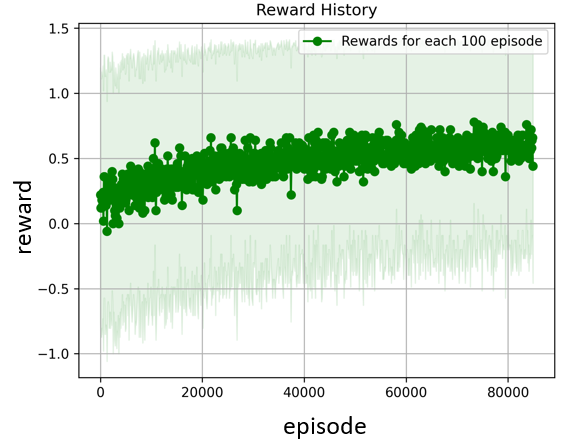
\includegraphics[width=150mm]{assets/MCS.eps}
  \caption{ステップ数10000の際の推移}
  \label{fig:MCS}
\end{figure}

\section{今後の課題}
今週の実験で大きなバグも現時点では見つからず, 1e6 程度のオーダーのエピソード数学習を行えばランダムに行動する相手に対して高い勝率を誇る AI を作成できることが分かった.
研究テーマが動的な難易度調整であるため,その方法とどのようなデータを取れば本研究の有効性や新規性が示せるかの検討をしなければならない.

\begin{figure}[htbp]
  \centering
  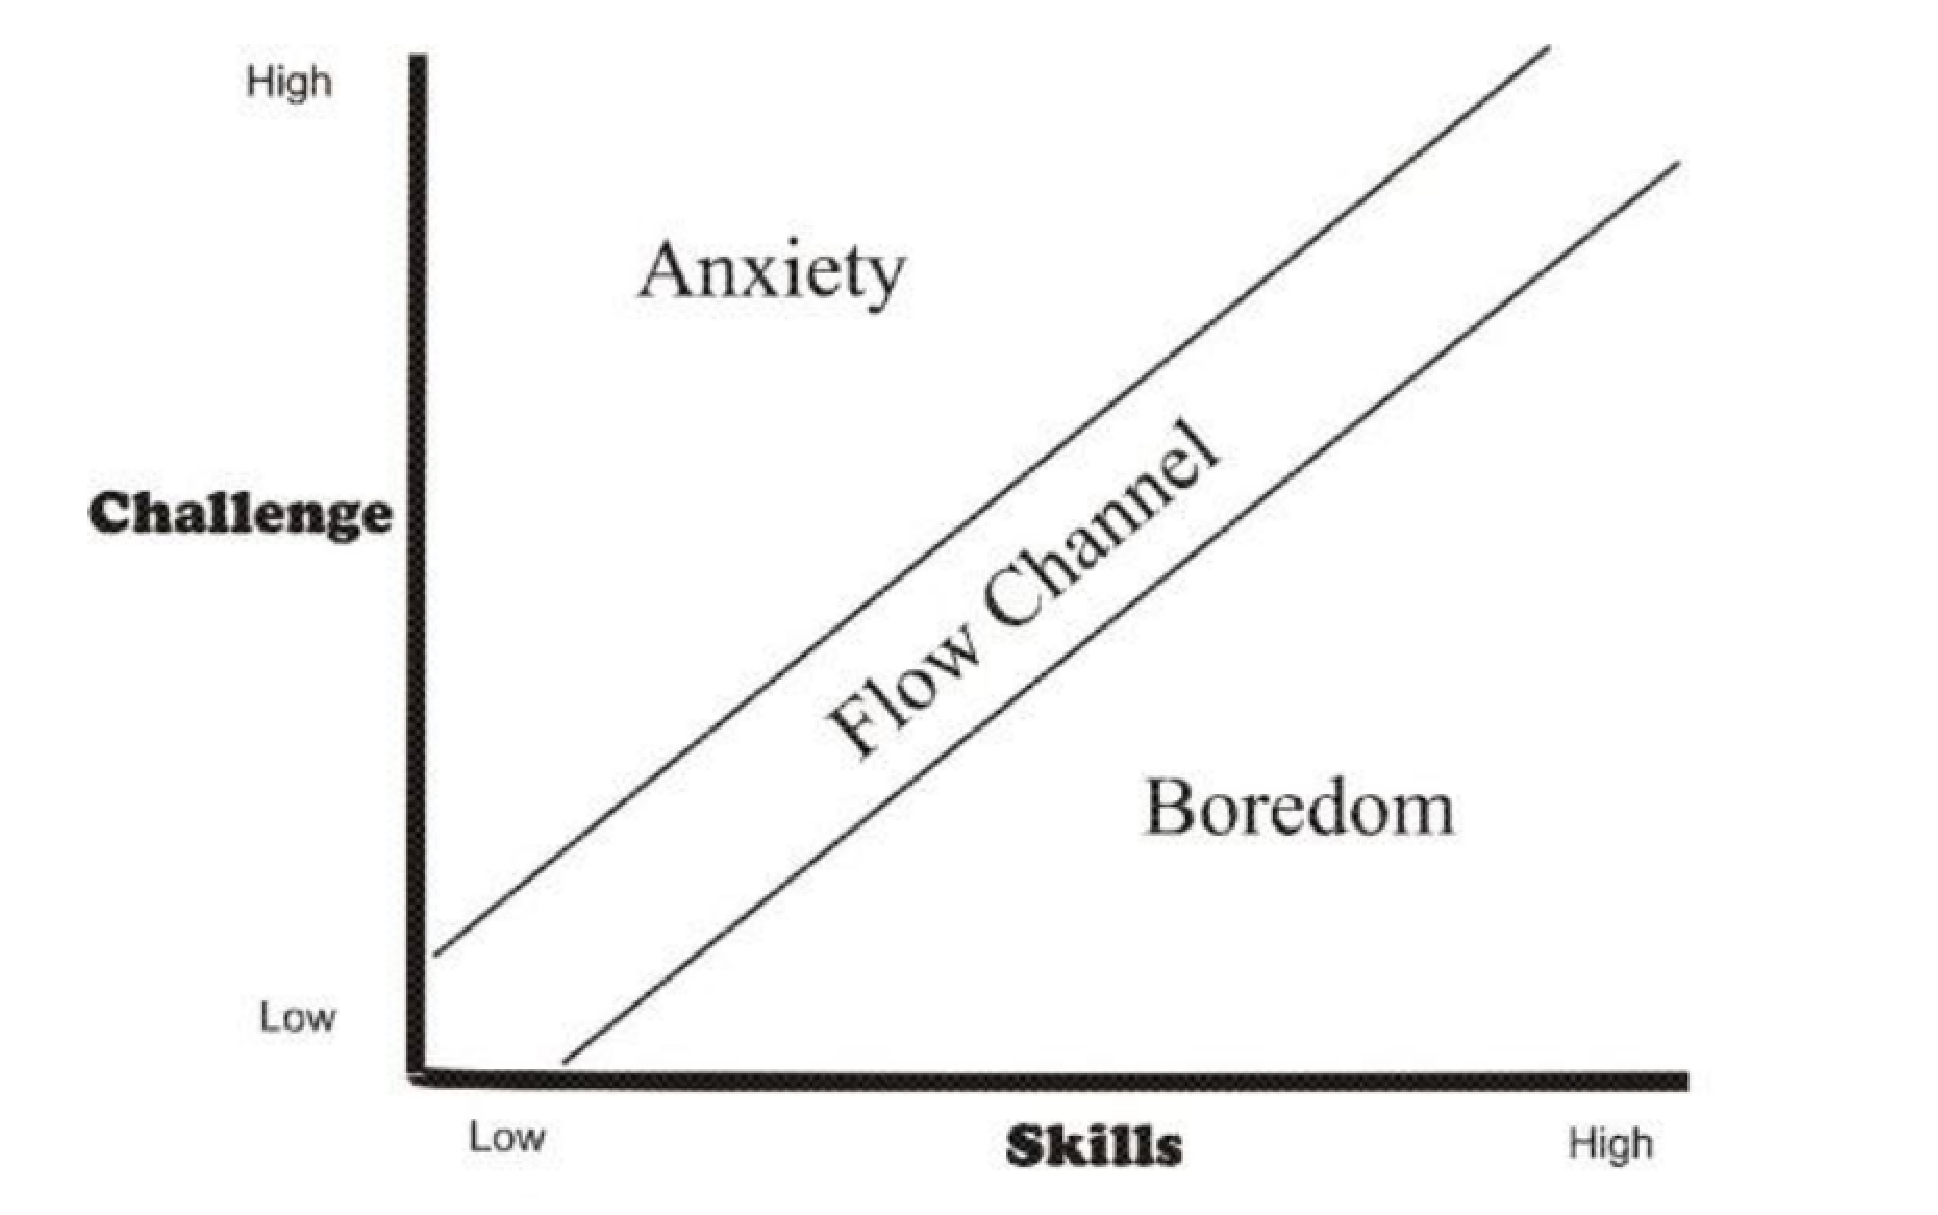
\includegraphics[width=150mm]{assets/Flow.eps}
  \caption{フローモデル}
  \label{fig:flow}
\end{figure}

動的難易度調整の研究は図 \ref{fig:flow} に示すフローモデルに基づいていることが多い.
フローとはユーザがある活動を実行しているときに,タスク実行中に没頭し,集中し,満たされた気持ちになる精神状態のことである.
プレイヤーをフロー内に維持し、退屈(課題が全くない)やフラストレーション(課題が難しすぎる)に達するのを避けるために、ゲームのレベルをコントロールすることが主な目的である\cite{DDA}.
難易度調整の際にはその都度プレイヤーが直面している状況の難易度を定義する必要があり,ヒューリスティックな知識を用いて評価関数を作成するか,プレイヤーのボディランゲージといったプレイヤーの人間の行動から判断するかの2種類がある\cite{DDA}.

ターン制のカードゲームの場合はどのような評価関数でプレイヤーが直面している難易度というものを定義すればよいのか,また敵カードのHP,攻撃力,プレイする枚数といったパラメータの中でどれを調整すればよいのか検討する必要がある.


%index.bibはtexファイルと同階層に置く
%ちゃんと\citeしないと表示されない(1敗)
\bibliography{index.bib}
\bibliographystyle{junsrt}

\end{document}